\documentclass[conference]{IEEEtran}

\usepackage{amsmath}
\usepackage{algorithmic}
\usepackage{graphicx}
\usepackage{textcomp}
\usepackage{xcolor}
\def\BibTeX{{\rm B\kern-.05em{\sc i\kern-.025em b}\kern-.08em
    T\kern-.1667em\lower.7ex\hbox{E}\kern-.125emX}}

% setup BibTex
\usepackage[
backend=biber,
style=ieee,
url=false,
isbn=false,
eprint=false
]{biblatex}
\addbibresource{references.bib}

% utility 
\usepackage{booktabs} % better tables
\usepackage{subcaption}
\usepackage{microtype}
\usepackage{comment}
\usepackage{siunitx}

% circuitikz
\usepackage[straightvoltages, american, europeanresistors, cuteinductors, RPvoltages]{circuitikz}

% cleverref, must be last
\usepackage[capitalise]{cleveref}
\begin{document}


\title{Effects of Compressive Stress on Ferrites in Inductive Power Transfer}

\author{
  Alexander K. Bailey, Jerry Sun\textsuperscript{\textdagger}, Wenting Zhang, Seho Kim, Willsen Wijaya\textsuperscript{\textdagger}, Tom Allen\textsuperscript{\textdagger}, Grant A. Covic\\
  \textit{Department of Electrical, Computer and Software Engineering}\\
  \textit{\textsuperscript{\textdagger}Centre for Advanced Materials Manufacturing and Design}\\
  \textit{University of Auckland}\\
  Auckland, New Zealand\\
  \{alexander.bailey, jerry.sun, wenting.zhang, seho.kim, willsen.wijaya, tom.allen, ga.covic\}@auckland.ac.nz\\ 
}
\maketitle

\begin{abstract}
  Inductive power transfer (IPT) magnetics are often `potted' with an encapsulant material to improve thermal performance.
  The difference in thermal expansion between common epoxy based encapsulant materials and ceramic ferrites creates a compressive load which permanently reduces the magnetic performance of the core material. 
  This article measures how the core loss of Mn--Zn ferrites changes with an applied compressive stress of \SIrange{10}{100}{\mega\pascal} at \SI{85}{\kilo\hertz}. 
  The measured data is used to predict how core losses change in a practical potted IPT pad, demonstrating a \textcolor{red}{\SI{140}{\percent}} increase in core loss. 
\end{abstract}

\begin{IEEEkeywords}
Core loss, inductive power transfer (IPT), loss measurement, magnetic losses
\end{IEEEkeywords}

\section{Introduction}

\IEEEPARstart{E}{lectric} vehicles (EVs) are increasingly common due to lowering costs and a rising need for climate change. 
However, existing infrastructure favours the outgoing Internal Combustion Engine Vehicles (ICEVs), meaning charging EVs can be cumbersome. 
Inductive power transfer (IPT) is a wireless charging technology that enables power transfer using magnetic fields. 
The application of this technology to the charging of EVs could enable more reliable and convenient charging of EVs of all power levels \cite{covicModernTrendsInductive2013b}. 

At higher power levels, thermal issues limit power density. 
In order to improve the thermal performance of the IPT magnetics, both the coil and core layer (shown in \cref{fig:padstructure}) are `potted' in an encapsulant material \cite{kneidlProcessingInfluencesResinbased2020}. 
Typical encapsulant materials have high thermal conductivity which improves the temperature profile uniformity and allows for a higher current density in the coil. 
However, several articles have noted the deterimental effect of encapsulant materials on the magnetic performance of ferrites. 

Polycrystalline ferrites show decreased magnetic permeability and a widening $B$-$H$ curve under applied pressure due to the compressed topography of the domain walls \cite{leflochEffectPressureSoft1981}. 
Foote et. al verified the reduction in permeability and increased core loss through the construction of a small-scale potted IPT coil assembly, demonstrating a \SI{\sim 100}{\percent} increase in losses \cite{footeEncapsulationResidualStress2023}.
This article aims to measure the effect of pressure on ferrite core loss at \SI{85}{\kilo\hertz} in a material independent and reproducable manner with standard core loss measurement techniques. that designers can better predict the impacts of encapsulation on the IPT system's behaviour. 

\begin{figure}[t]
  \centering
  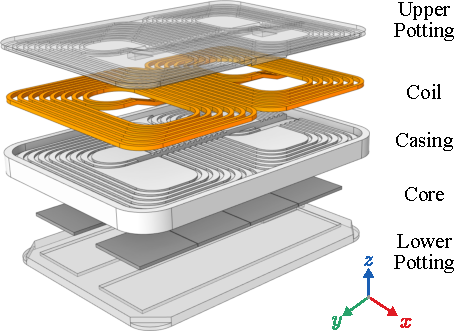
\includegraphics{figures/padstructure.pdf}
  \caption{Typical structure of IPT pad for EV charging}
  \label{fig:padstructure}
\end{figure}
\begin{figure}[t]
  \centering
  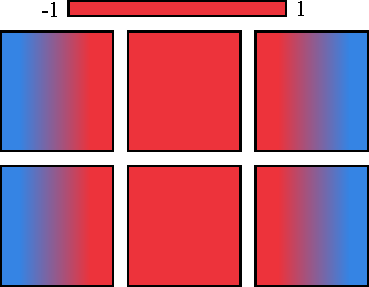
\includegraphics{figures/simulatedpottingpadstresses.pdf}
  \caption{FEA simulation of ambient residual stress on ferrites at \SI{25}{\celsius} after curing potting material at \SI{60}{\celsius}}
  \label{fig:pottingstresses}
\end{figure}

\section{Characterisation of Ferrite Under Stress}
Stress is a physical quantity that describes the forces acting on a material, simple uniaxial stress in the $z$ direction $\sigma_z$ can be calculated from, 
\begin{equation}
  \sigma_z = \frac{F_z}{A}
  \label{eqn:uniaxialstress}
\end{equation}
Where $F_z$ is the compressive force acting in the $z$ direction and $A$ is the cross-sectional area normal to the $z$-axis. 
Although the major stresses on ferrite tiles in IPT are shear (forces act to push layers of the material co-planar to each other), this article considers the material under compressive loading to simplify the measurement setup. 
The von Mises equivalent stress is a scalar value that represents the effect of each of the individual stress components, principal and shear, the von Mises equivalent stress $\sigma_\text{eqv}$ is used in this article to allow for comparisons between the measured compressive stress and the predicted shear stresses caused by the encapsulation material. 
By convention, compressive stress is negative and tensile stress is positive, however for simplicity, in this paper, compressive stress is considered positive unless the von Mises equivalent stress is used. 

For ferrites in IPT magnetics, the thermal strain occurs in two ways.
As shown in \cref{fig:pottingstresses}, when curing the potting material, residual stresses remain even after cooling down to room temperature. 
In operation, when the litz, ferrite and Aluminium plate heat up, each material will expand. 
When the coefficient of linear expansion $\alpha$ differs between two materials, the material exerts a force on the other. 
The $\alpha$ of ferrite is significantly lower than that of the surrounding encapsulation material creating compressive stresses exceeding \SI{100}{\mega\pascal}. 

\subsection{Methodology}

An Instron 1180R universal testing machine was used to apply a compressive force of up to \SI{200}{\kilo\newton} to the surface of toroid. 
However, in order to measure core loss in the hydraulic press, the toroid must be wound with two conductive windings. 
The designed fixture applies pressure to the surface of the toroid without impacting the litz wire.
\cref{fig:compressionholder} shows an overview of the designed setup. 

\begin{figure}
  \centering
  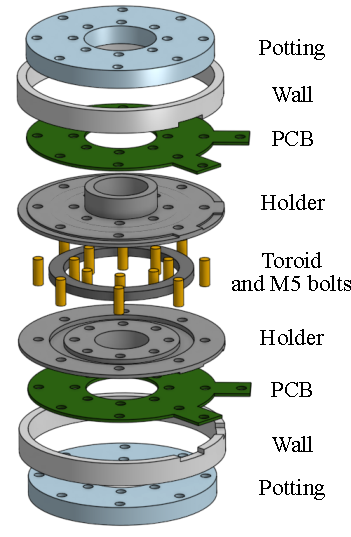
\includegraphics{figures/compressionholder.pdf}
  \caption{Exploded diagram of designed toroid compression setup}
  \label{fig:compressionholder}
\end{figure}

The designed fixture applies pressure to the surface where wire is not wound which creates a nonuniform pressure distribution on the surface. 
To simulate how the applied force was distributed across the toroid in this setup, a structural FEA simulation of the setup for each intended load was carried out. 
\cref{fig:holderfea} shows the predicted loads for \SI{100}{\kilo\newton} of compresive load, designed to apply a \SI{60}{\mega\pascal} compressive stress to the ferrite toroid.
From this simulation, the applied force is applied only to the areas without windings, in these areas the equivalent stress is almost zero. 
Hence, the equivalent stress in the toroid is not as predicted by \cref{eqn:uniaxialstress}. 

In addition, uniaxial compression does not result in purely compressive stress due to Poisson's effect, compression in the $z$ direction causes expansion in the $x$ and $y$ directions.
This creates tensile forces which causes brittle failure much before the ceramic material would fail under pure compression. 
Based on measurements from the literature, ferrite has a Poisson's ratio of approximately 0.25 \cite{moinuddinElasticBehaviourMnZn1993}.
This means that the applied stress deforms the ferrite toroid at approximately \SI{25}{\percent} the rate of compression in the $x$ and $y$ directions.

The nonuniform compression and influence of Poisson's effect means the stress-state of the toroid is more complex than pure compression and hence the predicted mean equivalent stress $\overline{\sigma_\text{eqv}}$ is used based on FEA simulations as shown in \cref{fig:holderfea}. 
The relevant material properties are given in \cref{sec:simulation}.

\begin{figure}
  \centering
  
\includegraphics{figures/holderfea.pdf}
  \caption{FEA of toroid under \SI{100}{\kilo\newton} compressive load}
  \label{fig:holderfea}
\end{figure}
\begin{table}
  \centering
  \caption{Toroid properties}
  \begin{tabular}{@{}llll@{}}
    \toprule
    Parameter & Value & Parameter & Value \\ \midrule
    Material & TDK N95 & $L_\text{p}$ & \textcolor{red}{\SI{5}{\micro\henry}} \\
    Inner Diameter & \SI{64}{\milli\meter} & $L_\text{s}$ & \textcolor{red}{\SI{5}{\micro\henry}} \\
    Outer Diameter & \SI{80}{\milli\meter} & $k$ & \textcolor{red}{$0.99$} \\
    $N_\text{p}$ & 4 & $R_\text{w,p}$ & \textcolor{red}{\SI{119}{\milli\ohm}} \\
    $N_\text{s}$ & 4 & $R_\text{w,s}$ & \textcolor{red}{\SI{119}{\milli\ohm}} \\
    \bottomrule
  \end{tabular}
  \label{tab:toroidproperties}
\end{table}

Toroids of TDK N95 ferrite were cut from \SI{5}{\milli\meter} tiles using a water jet cutter and wound with litz on the primary and magnet wire on the secondary. 
The toroid properties are given in \cref{tab:toroidproperties}.
The machining of ferrite has also been shown to increase core losses due to the mechanical stress imposed on the surface during the cutting process \cite{neumayrOriginQuantificationIncreased2019}. 
However, this effect is concentrated on the cut surface which for this case is the outer and inner surfaces, not in the mean flux path of the toroid hence the effects are expected to be minimal. 
Regardless, the following experiments include a factory-epoxy-coated R34 toroid of TDK N95 ferrite as a reference. 

For each mechanical loading scenario, the core loss $P_\text{core}$ was then measured using a partial cancellation method which modifies the conventional two-winding method with a compensation capacitor $C_s$ in series to cancel the reactive voltage across the inductor under test $L_t$ \cite{houNewHighFrequencyCore2017}. 
The equivalent circuit of this method is shown in \cref{fig:partialcancellationcircuit}.
$C_s$ could be selected to completely cancel the reactive power in the system, but maintaining resonance for different operating conditions is challenging. 
Instead, a partial cancellation method defines a voltage cancellation factor $k_v$, the ratio of the cancelled reactive voltage to the total reactive voltage, to only `partially' cancel the reactive component of $L_t$. 
In order to determine the value of $k_v$, a phase pertubation is introduced into $i_L$, creating \cref{eqn:pcoreprime}, $k_v$ can then be calculated by combining \cref{eqn:pcore} and \cref{eqn:pcoreprime}.
Using this method core loss was calculated from measurements of the current flowing through the primary winding $i_L(t)$, the voltage on the secondary winding $v_2(t)$ and the voltage across the compensation capacitor $v_C(t)$ by, 
\begin{equation}
  P_\text{core} = f \int_0^T v_2(t)i_L(t)dt + \frac{f}{k_v} \int_0^T v_c(t)i_L(t) dt
  \label{eqn:pcore}
\end{equation}
\begin{equation}
  P_\text{core}^{\prime} = f \int_0^T v_2(t)i_L^{\prime} (t)dt + \frac{f}{k_v} \int_0^T v_c(t)i_L^{\prime}(t) dt
  \label{eqn:pcoreprime}
\end{equation}
\begin{equation}
  k_v = \frac{\int_0^T v_c(t)i_L(t)dt - \int_0^T v_ci_L^\prime(t)dt}{\int_0^T v_2(t) i_L^\prime(t) dt - \int_0^T v_2(t) i_L(t) dt}
  \label{eqn:kv}
\end{equation}

\begin{figure}[t]
  \begin{subfigure}{\columnwidth}
    \centering
    \begin{circuitikz}
    \ctikzset{quadpoles style=inline}

    % Voltage source
    \draw (0,-3) to[sV, l=$V_\text{pa}$] (0,2);

    % I_L
    \draw (0,2) to[short, i^=$i_\text{L}(t)$] (1,2);

    % Winding resistance 
    \draw (1,2) to[R, R=$R_{w}$] (3,2);

    % Transformer
    \draw (6,2) node[transformer core, anchor=A1] (T) {}
      (T.A1) -- ++(-1.5,0) coordinate(TPa)
      (T.A2) to[short] ++(-1.5,0) coordinate(MDa);

    \draw (TPa) to[L, L=$L_\text{m}$] (MDa);
    \draw (TPa) to[short] ++(-1.5,0) coordinate(TP);
    \draw (MDa) to[short] ++(-1.5,0) coordinate(MD);
    \draw (TP) to[R=$R_\text{core}$] (MD);

    \draw (T.B1) -- ++(.5, 0) coordinate(TPb)
    to[open, v^<=$$, o-o] (TPb |- T.B2)
    -- (T.B2);

    % manually add v2 label
    \node[right] at (TPb -| T.B1) [xshift=0.5cm, yshift=-1.1cm] {$v_2(t)$};

  % Turns ratio label
    \node at ($(T.A1)!0.5!(T.B1)$) [above=0cm] {$N_p : N_s$};

    % Capacitor
    \draw (MD) to[C, a=$C_\text{s}$, v^=$v_C(t)$] (3,-3);

    \draw (3,-3) -- (0,-3);

    % Dashed box around Rw, Rcore, Lm, and transformer
    \draw[dashed] (1, 3) rectangle (8.3, -.5)
    node[above, midway, yshift=2cm, font=\itshape] {Wound toroid};

\end{circuitikz}

    \caption{}
    \label{fig:partialcancellationcircuit}
  \end{subfigure}
  \begin{subfigure}{\columnwidth}
    \centering
    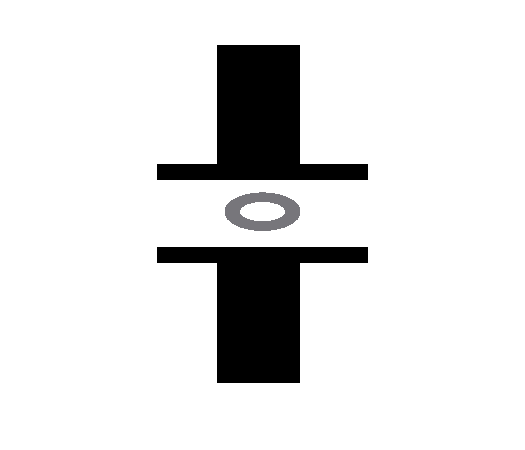
\includegraphics{figures/experimentalsetup.pdf}
    \caption{}
    \label{fig:experimentalsetup}
  \end{subfigure}
  \caption{(a) Equivalent circuit of the partial cancellation method, (b) Experimental setup for core loss measurement under compressive stress}
\end{figure}

\subsection{Results}

\cref{fig:BPcurves} shows the measured $B$-$P$ curve for each of the loading scenarios of the cut toroid and a reference manufacturer provided toroid. 
The unloaded cut toroid has slightly lower loss density than the manufacturer epoxied toroid, despite the stress-state from machining. 
This shows that the machined toroid is suitable for these measurements. 

The stress-dependent behaviour of ferrite has been shown to have a memory effect. 
After the compressive loading is removed, the permeability of the material is decreased and the core loss increases. 
In order to account for this, each sample is measured before, during and after loading. 
The results presented in \cref{fig:BPcurves} and \cref{fig:corelossstress} are all under active loading, 

\begin{figure}[t]
  \centering
  \begin{subfigure}{\columnwidth}
    \centering
    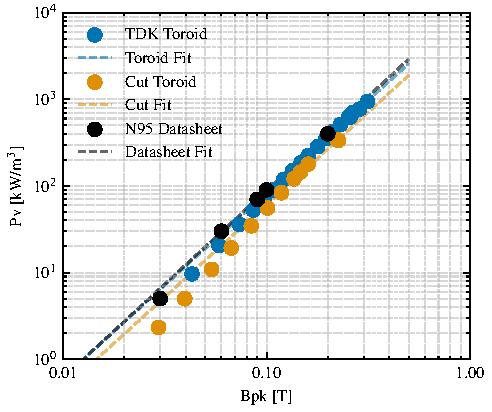
\includegraphics{figures/24-09-10_BP_curves.pdf}
    \caption{}
    \label{fig:BPcurves}
  \end{subfigure}
  \begin{subfigure}{\columnwidth}
    \centering
    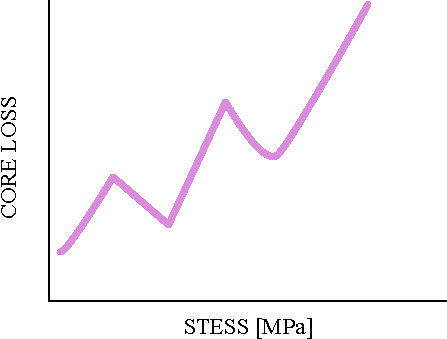
\includegraphics[width=3.5in, height=3in]{figures/coreloss.pdf}
    \caption{}
    \label{fig:corelossstress}
  \end{subfigure}
  \caption{(a) $B$-$H$ curves of the TDK N95 ferrite toroid under several levels of compressive loading $\overline{\sigma_\text{eqv}}$, (b) Core loss of TDK N95 ferrite toroid under several levels of compressive loading at \SI{\sim 5}{\milli\tesla}, \SI{\sim 25}{\milli\tesla}, \SI{\sim 50}{\milli\tesla} and \SI{\sim 100}{\milli\tesla}, \SI{85}{\kilo\hertz}}
\end{figure}
pressure
\section{Verification of Core Loss Measurements}
\label{sec:simulation}

This section presents two experiments which verify the measured results from the previous section. 
Firstly, three toroids of TDK N95 ferrite were potted with different encapsulation materials and the measured core loss compared to FEA simulations using the measured data. 
Finally, the core loss of a constructed Double D IPT pad is compared before and after potting, and the core loss after potting is predicted using the measured results. 

\subsection{Potted Toroid Measurement}

In order to verify the accuracy of the structural FEA simulations, three toroids of the same dimensions as described in the previous section were potted with different materials.
The potted toroids and the FEA predicted equivalent stress is shown in \cref{fig:pottedtoroids}.
The harder encapsulation materials show high residual stresses and hence higher core loss. 
However, the designer must trade off the desired mechanical behaviour of the encapsulation material and the effect of the encapsulation material on the system core losses. 

\begin{figure*}
  \centering
  \begin{subfigure}{\textwidth}
    \begin{subfigure}{0.3\textwidth}
      \centering
      
\includegraphics{figures/toroid.pdf}
      \caption{UR5608}
    \end{subfigure}~
    \begin{subfigure}{0.3\textwidth}
      \centering
      
\includegraphics{figures/toroid.pdf}
      \caption{PX900D}
    \end{subfigure}~
    \begin{subfigure}{0.3\textwidth}
      \centering
      
\includegraphics{figures/toroid.pdf}
      \caption{ER2223}
    \end{subfigure}

    \begin{subfigure}{0.3\textwidth}
      \centering
      
\includegraphics{figures/featoroid.pdf}
      \caption{}
    \end{subfigure}~
    \begin{subfigure}{0.3\textwidth}
      \centering
      
\includegraphics{figures/featoroid.pdf}
      \caption{}
    \end{subfigure}~
    \begin{subfigure}{0.3\textwidth}
      \centering
      
\includegraphics{figures/featoroid.pdf}
      \caption{}
    \end{subfigure}
  \end{subfigure}
  \caption{Experimental potted toroids and FEA structural simulations}
  \label{fig:pottedtoroids}
\end{figure*}

\begin{table}
  \centering
  \caption{Mechanical properties of relevant materials}
  \begin{tabular}{@{}llll@{}}
    \toprule
    Material & Manufacturer & $\alpha$ $\times 10^{-6}$ & $Y$ \\ \midrule
    N95 Ferrite & TDK & $10$ & \SI{119}{\giga\pascal} \\
    Nylon & TDK & $10$ & \SI{119}{\giga\pascal} \\
    FR4 PCB & TDK & $10$ & \SI{119}{\giga\pascal} \\
    UR5608 & TDK & $10$ & \SI{119}{\giga\pascal} \\
    PX900D & TDK & $10$ & \SI{119}{\giga\pascal} \\
    ER2223 & TDK & $10$ & \SI{119}{\giga\pascal} \\
    \bottomrule
  \end{tabular}
\end{table}

\subsection{Core Loss Prediction of Potted IPT Pad}
The core loss of a Double D IPT pad designed for \textcolor{red}{\SI{11}{\kilo\watt}} was measured using the stepped resonance method described in \cite{kalraPowerLossMeasurement2020}.
At rated current, the unpotted pad showed a total loss of \textcolor{red}{\SI{0}{\watt}}, with \textcolor{red}{\SI{0}{\watt}} of core loss.
When potted in two pours with UR5608, the total loss increased to \textcolor{red}{\SI{0}{\watt}} with \textcolor{red}{\SI{0}{\watt}} of core loss. 
\cref{fig:pottingstresses} shows an FEA simulation of the stress induced by this potting process. 
Use the predicted equivalent stress in the ferrites, the Steinmetz coefficients for each ferrite tile were adjusted accordingly and the core loss distribution shown in \cref{fig:padcoreloss} was predicted. 
The FEA simulation predicted a core loss of \textcolor{red}{\SI{0}{\watt}}, an error of \textcolor{red}{\SI{0}{\percent}}. 
\begin{figure}[t]
  %\includegraphics[width=3.5in, height=2in]{figures/padcoreloss}
  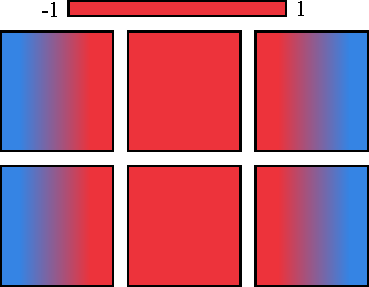
\includegraphics[width=3.5in, height=2in]{figures/simulatedpottingpadstresses.pdf}
  \caption{Predicted core loss distribution in DD pad under \textcolor{red}{\SI{30}{\kilo\volt\ampere}} operation considering thermal and structural impacts on the ferrites}
  \label{fig:padcoreloss}
\end{figure}

\section{Conclusion}

\section*{References}
\printbibliography[heading=none]

\end{document}
